\section{Detalle Primera Iteración}

\subsection{Detalle y tareas de casos de uso}

A continuación se presenta una descripción de alto nivel de los casos de uso a 
desarrollar durante la primera iteración. Además, se define la lista de tareas 
relacionadas con cada CU.

\subsubsection{\underline{CU01: Enviando información del vehículo al servidor}}

Detalle: Se refiere a la acción de mandar los datos obtenidos por el gps de los 
vehículos al servidor de forma segura.


Tareas: 
\begin{itemize}

\item CU01-T01: Analizar volumen de datos

\item CU01-T02: Investigacion de tecnologias
\begin{itemize}
\item CU01-T02-st01: Seguridad
\item CU01-T02-st02: Concurrencia
\item CU01-T02-st03: Alto rendimiento
\end{itemize}

\item CU01-T03: Investigación de formas de comunicación
\begin{itemize}
\item CU01-T03-st01: Internet
\item CU01-T03-st02: Radiofrecuencia
\item CU01-T03-st03: GSM
\item CU01-T03-st04: Satelital (ArSAT)
\end{itemize}

\item CU01-T04: Configuración del ambiente de desarrollo 
\item CU01-T05: Especificación de la información necesaria para generar las infracciones 
\item CU01-T06: Implementación de mock del dispositivo del vehículo 
\item CU01-T07: Configuración del ambiente de testing 
\item CU01-T08: Testing 

\end{itemize}

\begin{table}[htb]
\begin{center}
\begin{tabular}{|l|c|}
\hline
Tarea & Estimación (Horas Hombre) \\
\hline \hline
CU01-T01: Analizar volumen de datos & 2 \\ \hline
CU01-T02: Investigacion de tecnologias & 10 \\ \hline
CU01-T03: Investigación de formas de comunicación & 10 \\ \hline
CU01-T04: Configuración del ambiente de desarrollo & 4 \\ \hline
CU01-T05: Especificación de la información necesaria para generar las infracciones & 4 \\ \hline
CU01-T06: Implementación de mock del dispositivo del vehículo & 4 \\ \hline
CU01-T07: Configuración del ambiente de testing & 4 \\ \hline
CU01-T08: Testing & 16 \\ \hline \hline
Total HH & 54 \\ \hline
\end{tabular}
\caption{Estimación de tiempo en horas hombre de las tareas del CU01}
\end{center}
\end{table}


\begin{figure}
  \centering
    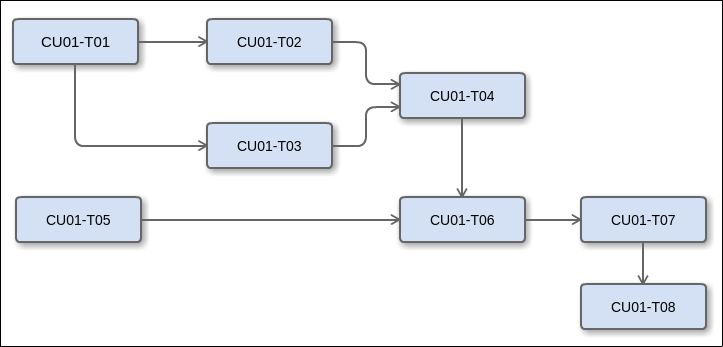
\includegraphics[width=1\textwidth]{./imagenes/dependenciasCU01.png}
  \caption{Grafo de dependencias entre tareas del CU01}
\end{figure}


\subsubsection{\underline{CU02: Detectando baja conectividad}}

Detalle: Se refiere a la acción de localizar las zonas en las cuales no hay buena 
conectividad, avisando al sistema ManejAR.


Tareas: 
\begin{itemize}

\item CU02-T01: Investigación de tecnologías para sensores
\begin{itemize}
\item CU02-T01-st01: Hardware
\item CU02-T01-st02: Software
\end{itemize}

\item CU02-T02: Implementar comunicación de los sensores con los servidores

\item CU02-T03: Implementar algoritmos de nivel de conectividad en el servidor 
\begin{itemize}
\item CU02-T03-st01: Definir qué se considera baja conectividad
\item CU02-T03-st02: Implementar algoritmo
\end{itemize}

\item CU02-T04: Implementación de mock del dispositivo de los sensores
\item CU02-T05: Implementar una demo para la empresa de Drones
\item CU02-T06: Configuración del ambiente de testing
\item CU02-T07: Testing

\end{itemize}

\begin{table}[htb]
\begin{center}
\begin{tabular}{|l|c|}
\hline
Tarea & Estimación (Horas Hombre) \\
\hline \hline
CU02-T01: Investigación de tecnologías para sensores & 6 \\ \hline
CU02-T02: Implementar comunicación de los sensores con los servidores & 16 \\ \hline
CU02-T03: Implementar algoritmos de nivel de conectividad en el servidor & 8 \\ \hline
CU02-T04: Implementación de mock del dispositivo de los sensores & 4 \\ \hline
CU02-T05: Implementar una demo para la empresa de Drones & 16 \\ \hline
CU02-T06: Configuración del ambiente de testing & 4 \\ \hline
CU02-T07: Testing & 12 \\ \hline \hline
Total HH & 66 \\ \hline
\end{tabular}
\caption{Estimación de tiempo en horas hombre de las tareas del CU02}
\end{center}
\end{table}


\begin{figure}	
  \centering
    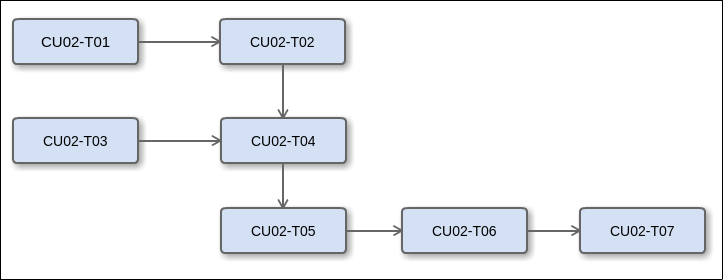
\includegraphics[width=1\textwidth]{./imagenes/dependenciasCU02.png}
  \caption{Grafo de dependencias entre tareas del CU02}
\end{figure}


\newpage

\subsection{Tareas de la primera iteración}

\begin{itemize}
\item Identificador de iteración: E01
\item Tipo de iteración: Elaboración
\item Tareas:
\begin{itemize}
\item E01-T01: Diseño conceptual del sistema 
\item E01-T02: Realización de WBS 
\item E01-T03: Análisis de riesgos 
\item E01-T04: Refinamiento de objetivos y requerimientos 
\item E01-T05: Reconocimiento de casos de uso
\item E01-T06: Priorización de casos de uso
\item E01-T07: Estimación de tiempo de casos de uso 
\item E01-T08: Análisis de atributos de calidad del sistema 
\item E01-T09: Diseño de arquitectura del sistema 
\item E01-T010: Elección de tecnologías 
\item E01-T011: Realización de las tareas del caso de uso CU01 - Enviando información del vehículo al servidor 
\item E01-T012: Realización de las tareas del caso de uso CU02 - Detectando baja conectividad 
\end{itemize}
\end{itemize}


\begin{table}[htb]
\begin{center}
\begin{tabular}{|l|c|}
\hline
Tarea & Estimación (Horas Hombre) \\
\hline \hline
E01-T01: Diseño conceptual del sistema & 16 \\ \hline
E01-T02: Realización de WBS & 8 \\ \hline
E01-T03: Análisis de riesgos & 2 \\ \hline
E01-T04: Refinamiento de objetivos y requerimientos & 16 \\ \hline
E01-T05: Reconocimiento de casos de uso & 6 \\ \hline
E01-T06: Priorización de casos de uso & 1 \\ \hline
E01-T07: Estimación de tiempo de casos de uso & 1 \\ \hline
E01-T08: Análisis de atributos de calidad del sistema & 12 \\ \hline
E01-T09: Diseño de arquitectura del sistema & 128 \\ \hline
E01-T010: Elección de tecnologías & 16 \\ \hline
E01-T011: Realización de las tareas del caso de uso CU01 - \\ Enviando información del vehículo al servidor & 54 \\ \hline
E01-T012: Realización de las tareas del caso de uso CU02 - \\ Detectando baja conectividad & 66 \\ \hline \hline
Total HH & 326 \\ \hline
\end{tabular}
\caption{Estimación de tiempo en horas hombre}
\end{center}
\end{table}


\subsection{Gantt de la primera iteración}

A continuación se muestra el gráfico del gantt resultante.
Los recursos son los cuatro integrantes del equipo.
\newline

\centerline{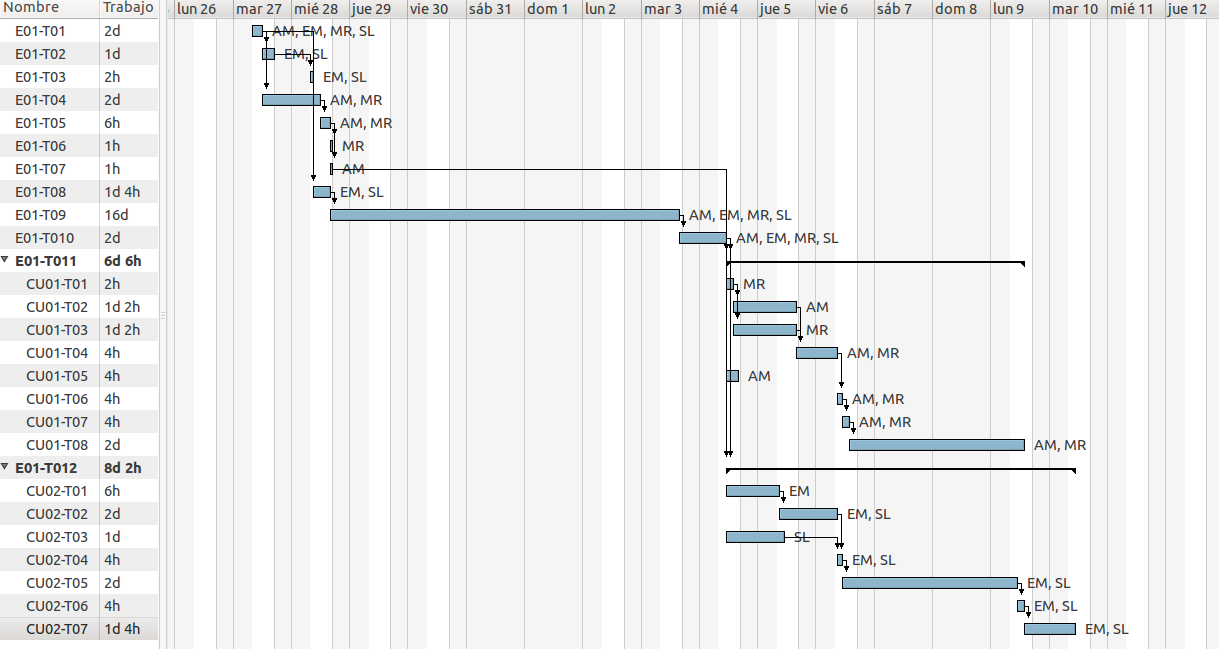
\includegraphics[width=1\textwidth]{./imagenes/gantt.png}}
